\section{\label{sec:level1}Experimental Setup}
The measurements used for this analysis was taken with the \abbr{CLAS} detector at Hall B at the Thomas Jefferson National Accelerator Facility \abbr{TJNAF} located in Newport News, Virginia. The \g12 experiment ran during March - June 2008 with a total of 44 days of good beam time. It collected over 128~TB of raw data that consisted of $26\cdot 10^9$ events, with an integrated luminosity of 68~pb$^{-1}$. A detailed explanation of the \abbr{CLAS} data reconstruction and explanation of the \abbr{DAQ} for \g12 can be found in~\cite{clas.g12.note}. This chapter will briefly overview aspects of the \g12 running conditions and data retrieval found in~\cite{clas.g12.note}.
\subsection{\g12 Data Acquisition and Triggering  }\label{sec:clas.g12.conditions.data}

The \clas  detector is comprised of several subsystems. Each subsystem in \clas has its own electronics package to monitor its components and collect signals. Discriminators determine whether a signal each each channel a subsystem exceeds a given threshold. In the case of the \abbr{DC} the signal is supplied from the sense wire. For the \abbr{ST}, \abbr{CC}, \abbr{TOF}, \abbr{EC} subsystems, the signal is supplied by converting the current supplied by an anode of a \abbr{PMT} or cluster of \abbr{PMT}'s into a voltage. Each subsystem has a preset voltage threshold. The discriminator compares the signal output of a subsystem to the preset threshold. Signals that exceed the preset threshold are digitized by two types of hardware, Time-to-digital converters (\abbr{TDC}s) and Analog-to-digital converters (\abbr{ADC}s). \abbr{TDC}s report the time at which a signal arrives, while \abbr{ADC}s report a number corresponding to the integral of the signal.

The presence of a signal in a single subsystem does not constitute a physics event. There are a number of unwanted sources that could produce unwanted signals, such as cosmic radiation, electronic noise, Fano noise etc. It is the job of the trigger to determine which sets of signals constituted a physics event. The trigger is a list of signals from various subsystems required for an event to be written out to disk. An item in the trigger list is known as a trigger ``bit''. The \g12 rungroup used a field-programmable gate array (\abbr{FPGA}) as the trigger supervisor. The \abbr{FPGA} allowed for 12 independent trigger configurations to be employed at one time during the running of \g12 as well as the ability to change the trigger configuration during running. The detector subsystems used in the first-level (\abbr{L1}) triggering system of \g12 are the \abbr{TAGR}, \abbr{ST},  \abbr{CC}, \abbr{TOF}, and \abbr{EC}. The \abbr{TOF} and \abbr{ST} are used to identify charged tracks, at the trigger level, by using coincidence of any one \abbr{TOF} hit in a given sector with any one \abbr{ST} hit in the same sector. Also, a coincidence between the \abbr{EC} and \abbr{CC} was included as a lepton trigger. Fig.~\ref{fig:clas.daq.trigsec} depicts the \abbr{L1} trigger configuration for the subsystems mentioned except for the \abbr{TAGR} subsystem. During the \g12 experiment, the interval for a trigger coincidence was 100 ns. All subsystems of \clas except for the \abbr{DC} can acquire signals in a few nanoseconds.
\begin{figure}[h]\begin{center}
		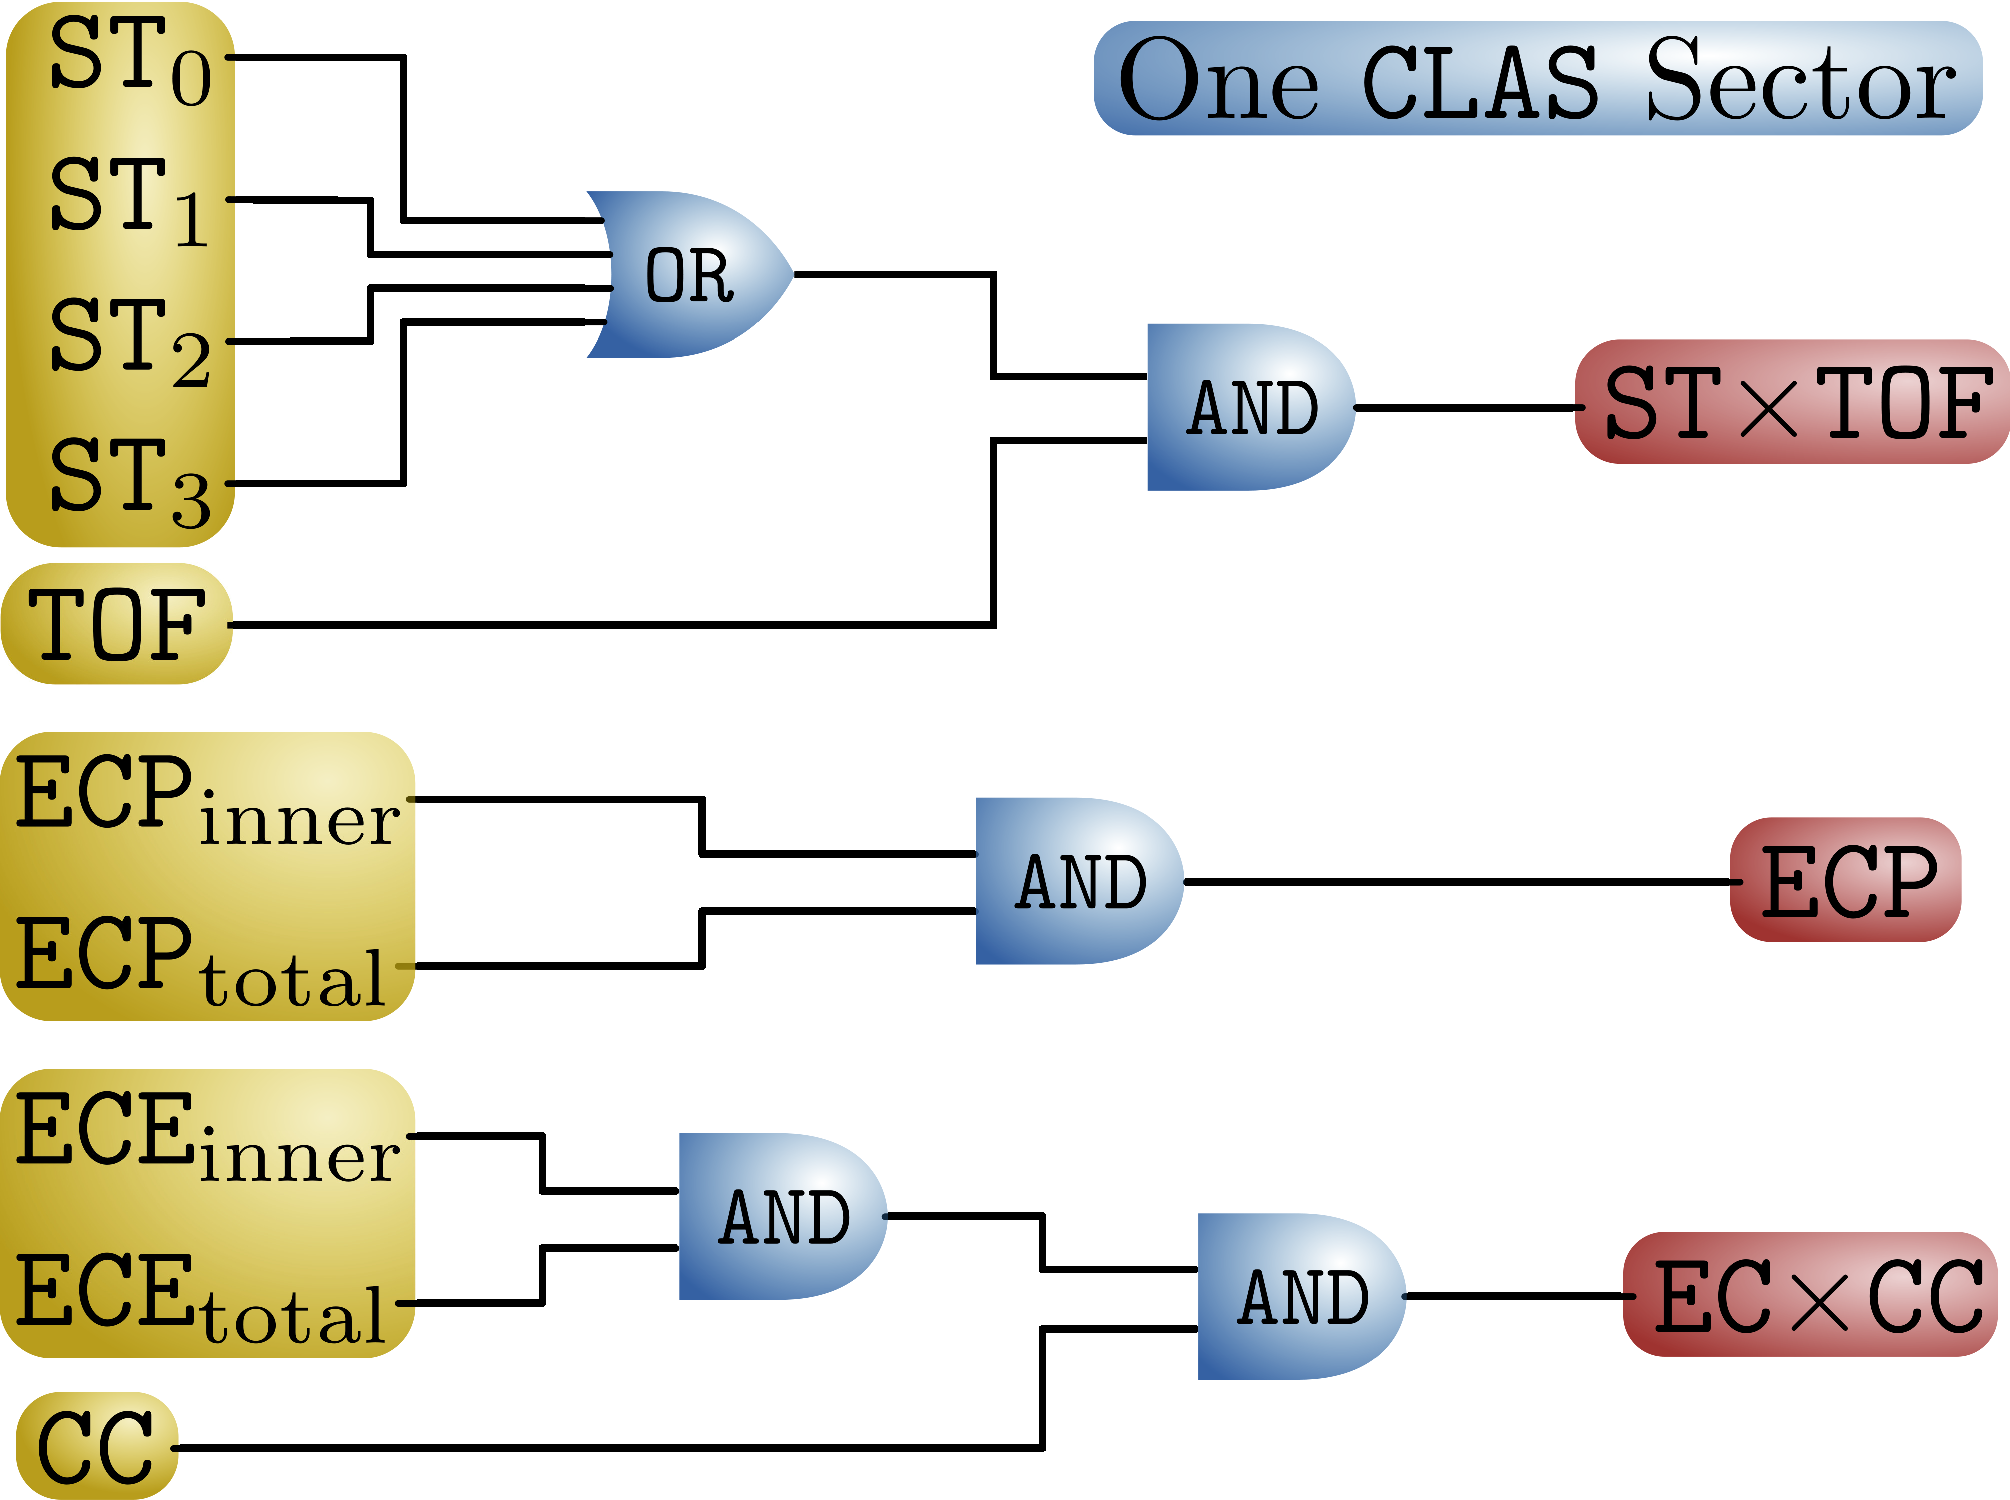
\includegraphics[width=0.8\figwidth]{\figures/hall-b/trigger_sector.pdf}
		\caption[Trigger logic for one of the six sectors of \abbr{CLAS}]{\label{fig:clas.daq.trigsec}{\coloronline}Trigger logic for one of the six sectors of \abbr{CLAS}. The \abbr{ST$\times$TOF} signal is a coincidence between any of the four start counter \abbr{TDC} signals (numbered from 0 to 3) and any of the 57 \abbr{TOF} \abbr{TDC} signals. The \abbr{ECE}$_\mathrm{inner}$ and \abbr{ECE}$_{\mathrm{total}}$ are the electron-threshold \abbr{EC} signals for the energy deposited in the \emph{inner} layer and in \emph{all} layers. These are combined with a \abbr{CC} signal to produce the \abbr{EC$\times$CC} trigger for this sector. The \abbr{ECP} trigger signal is the photon-threshold \abbr{EC} signal. These trigger signals are discussed further in Sec.~\ref{sec:data.trig}.}
	\end{center}\end{figure}
	
	When a first-level trigger requirement is satisfied, a second-level (\abbr{L2}) trigger requirement is sometimes necessary to verify the \abbr{L1} trigger. A \abbr{L2} trigger is usually a software routine unlike the \abbr{L1} trigger which is based on hardware. The \abbr{L2} trigger is typically employed for measurements from the \abbr{DC} and is slower than the \abbr{L1} trigger because it is software based. The software routine does coarse track reconstruction on the \abbr{DC} hits to confirm that the L1 coincidence was caused by particles traveling through \clas rather than unwanted noise.
	
	When a trigger configuration is completely satisfied, the data acquisition system (\abbr{DAQ}) collected the signals and wrote them to magnetic tape for future offline analysis. At the time \g12 was run, the \abbr{DAQ} was capable of running at 8~kHz.
	
	\subsubsection{\g12 Trigger Configuration} \label{sec:data.trig}
	The trigger configuration used in the \g12 running period are listed in Tables~\ref{tab:data.trig.conf.1}, \ref{tab:data.trig.conf.2} and \ref{tab:data.trig.conf.3}. All but one ``bit'' required a (\abbr{ST}$\cdot$\abbr{TOF}) to be present along with other requirements. The (\abbr{ST}$\cdot$\abbr{TOF}) configuration required a track to have coincidence in one sector between any one of the four start counter paddles of that sector, and any one of the 57 time-of-flight paddles in the same sector. Any configuration listed in the Tables~\ref{tab:data.trig.conf.1}, \ref{tab:data.trig.conf.2} and \ref{tab:data.trig.conf.3} with the suffix ``$\times$ N'' after a parenthesis grouped configuration requires that given configuration to have ``N'' coincidences in different sectors. To illustrate this the configuration (\abbr{ST}$\cdot$\abbr{TOF}) requires one coincidence in the same sector, while (\abbr{ST}$\cdot$\abbr{TOF})$\times$ 2 requires two coincidences of (\abbr{ST}$\cdot$\abbr{TOF}) in two different sectors and (\abbr{ST}$\cdot$\abbr{TOF})$\times$ 3 requires three coincidences of (\abbr{ST}$\cdot$\abbr{TOF}) in three different sectors. The hardware and configuration did not allow triggering of two tracks in the same sector because there were only six signals coming from the \abbr{TOF}, one for each sector. 
	
	Another component that can be included into a trigger ``bit'' is ``Master-\abbr{OR},'' (\abbr{MOR}). This component is a signal with the photon tagger. These are defined in Table~\ref{tab:data.trig.mor} and is illustrated with the other components of a ``bit'' in Fig.~\ref{fig:clas.daq.triglogic}.
	\begin{figure}[h]\begin{center}
			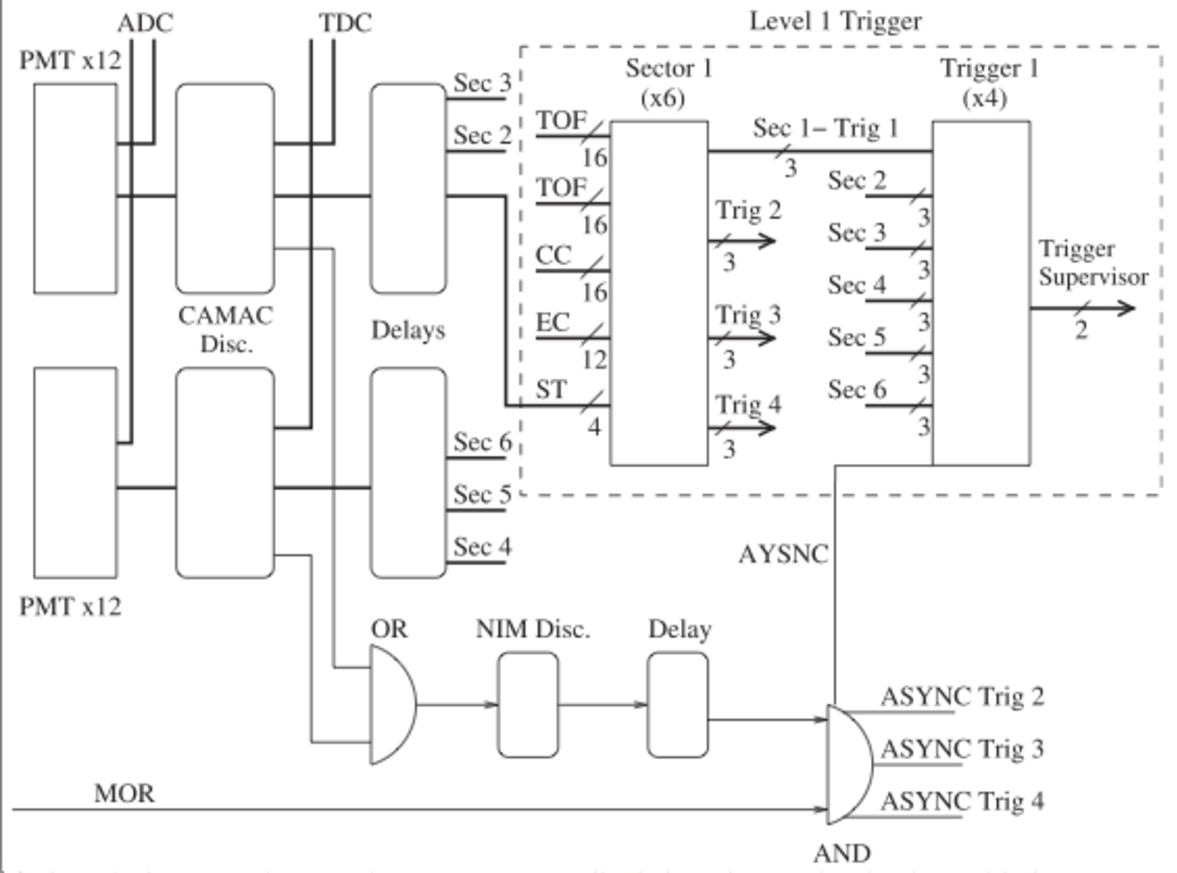
\includegraphics[width=0.8\figwidth]{\figures/hall-b/trigger_logic_w_st.pdf}
			\caption[Trigger logic for any of the six sectors of \abbr{CLAS} along with \abbr{MOR} asynchronous logic trigger input]{\label{fig:clas.daq.triglogic}{\coloronline}Trigger logic for any of the six sectors of \abbr{CLAS} along with \abbr{MOR} asynchronous logic trigger input.}
		\end{center}\end{figure}
		
		\subsubsection{Lepton Triggering and Neutral Triggering}\label{sec.data.trig.lepton}
		In \g12, since the \abbr{CC} was filled with gas, it was possible to include the \abbr{CC} as a component of the trigger. 
		There were three trigger ``bits'' used for lepton identification in \g12 as listed in Table~\ref{tab:data.trig.conf.2}. Each ``bit'' used a (\abbr{EC}$\cdot$\abbr{CC}) configuration to identify leptons. The (\abbr{EC}$\cdot$\abbr{CC}) configuration required a coincidence between the electromagnetic calorimeter and the Cherenkov subsystems. This coincidence was established by using the voltage sum of the \abbr{CC} for a sector and the voltage sum of the \abbr{EC} for the same sector and comparing each sum to a preset threshold described in Table~\ref{tab:data.ecccthresh}. The \abbr{EC} voltage sum threshold comparison is done on both the \abbr{EC}$_\mathrm{inner}$ and \abbr{EC}$_{\mathrm{total}}$ which are the \abbr{EC} voltage signals for the energy deposited in the inner layer and in all layers. The labels of photon or electron specified in Table~\ref{tab:data.ecccthresh} are not actual photons or electrons, but were considered a first-order approximation for detection. The particle identification is done at the analysis level. The method for determining the (\abbr{EC}$\cdot$\abbr{CC}) does not allow for multiple lepton triggering in the same sector. Determining multiple leptons in the same sector is done at the analysis level. 
		
		The ``bit 6'' trigger configuration, (\abbr{ST}$\cdot$\abbr{TOF})$\cdot$(\abbr{EC}$\cdot$\abbr{CC}) requires a \abbr{ST} and \abbr{TOF} coincidence previously described in~\ref{sec:data.trig} along with a coincidence between the electromagnetic calorimeter and the Cherenkov subsystems described above. The (\abbr{ST}$\cdot$\abbr{TOF}) configuration of ``bit 6'' did not have to be in the same sector as the (\abbr{EC}$\cdot$\abbr{CC}) configuration of ``bit 6''. The ``bit 11'' trigger configuration, (\abbr{EC}$\cdot$\abbr{CC})$\times$2 requires two coincidences between the electromagnetic calorimeter and the Cherenkov subsystems described above, in two different sectors. 
		
		The ``bit 5'' trigger configuration was also established as a lepton trigger. It required \abbr{EC} hits in two sectors. The ``bit 5'' trigger configuration was also established to analyze physics involving two or more neutral particles accompanied with a charged track, such as exclusive \piz production in which the \piz decays via 2 photons. The method for ``bit 5'' voltage sum comparison is identical to the \abbr{EC} voltage sum of ``bit 6'' and ``bit 11''
		
		It should be noted that none of the lepton triggers required a \abbr{MOR} signal, allowing for physics involving leptons to be measured starting from \g12's lowest tagger detection value of 1.142~GeV.
		
%		\begin{table}
\begin{minipage}{\textwidth}
\begin{center}
\begin{singlespacing}

\caption[Trigger Configuration 1]{\label{tab:data.trig.conf.1}Trigger configuration for \g12 runs from 56363 to 56594 and 56608 to 56647. (\abbr{ST}$\cdot$\abbr{TOF})$_{i}$ indicates a trigger-level track defined as a coincidence between a start counter and time-of-flight hit in the \ith\ sector. \abbr{MORA} and \abbr{MORB} represent coincidences with tagger hits within a certain energy range as specified in Table~\ref{tab:data.trig.mor}.}

\begin{tabular}{cccc}

\hline

\multicolumn{4}{c}{\g12 runs 56363--56594, 56608--56647} \\

\hline

bit & definition & L2 multiplicity & prescale \\

\hline

1 & \abbr{MORA}$\cdot$(\abbr{ST}$\cdot$\abbr{TOF})$_{1}\cdot$(\abbr{ST}$\cdot$\abbr{TOF})$_{i\neq 1}$ & -- & 1 \\
2 & \abbr{MORA}$\cdot$(\abbr{ST}$\cdot$\abbr{TOF})$_{2}\cdot$(\abbr{ST}$\cdot$\abbr{TOF})$_{i\neq 2}$ & -- & 1 \\
3 & \abbr{MORA}$\cdot$(\abbr{ST}$\cdot$\abbr{TOF})$_{3}\cdot$(\abbr{ST}$\cdot$\abbr{TOF})$_{i\neq 3}$ & -- & 1 \\
4 & \abbr{MORA}$\cdot$(\abbr{ST}$\cdot$\abbr{TOF})$_{4}\cdot$(\abbr{ST}$\cdot$\abbr{TOF})$_{i\neq 4}$ & -- & 1 \\
5 & \abbr{MORA}$\cdot$(\abbr{ST}$\cdot$\abbr{TOF})$_{5}\cdot$(\abbr{ST}$\cdot$\abbr{TOF})$_{i\neq 5}$ & -- & 1 \\
6 & \abbr{MORA}$\cdot$(\abbr{ST}$\cdot$\abbr{TOF})$_{6}\cdot$(\abbr{ST}$\cdot$\abbr{TOF})$_{i\neq 6}$ & -- & 1 \\
7 & \abbr{ST}$\cdot$\abbr{TOF} & -- & 1 \\
8 & \abbr{MORA}$\cdot$(\abbr{ST}$\cdot$\abbr{TOF})$\times$2 & -- & 1 \\
11\footnote{bit 11 and \abbr{MORB} were included in the trigger starting with run 56519.} & \abbr{MORB}$\cdot$(\abbr{ST}$\cdot$\abbr{TOF})$\times$2 & -- & 1 \\
12 & (\abbr{ST}$\cdot$\abbr{TOF})$\times$3 & -- & 1 \\

\hline \hline

\end{tabular}

\end{singlespacing}
\end{center}
\end{minipage}
\end{table}
\vspace{20pt}
 % label: tab:data.trig.conf.1
%		
%		\begin{table}
\begin{minipage}{\textwidth}
\begin{center}
\begin{singlespacing}

\caption[Trigger Configuration 2]{\label{tab:data.trig.conf.2}Trigger configuration for \g12 runs from 56595 to 56607 and 56648 to 57323. \vspace{0.75mm}}

\begin{tabular}{cccc}

\hline

\multicolumn{4}{c}{\g12 runs 56595--56607, 56648--57323 } \\

\hline

bit & definition & L2 multiplicity\footnote{Level 2 triggering was turned off on all bits for runs 56605, 56607 and 56647.} & prescale \\

\hline

1 & \abbr{MORA}$\cdot$(\abbr{ST}$\cdot$\abbr{TOF}) & 1 & 1000/300\footnote{Prescaling for bits 1 and 4 were 1000 for runs prior to 56668 at which point they both were changed to 300.} \\
2 & \abbr{MORA}$\cdot$(\abbr{ST}$\cdot$\abbr{TOF})$\times$2 & 2/--\footnote{Level 2 triggering of bit 2 was set to 2 for runs prior to 56665 at which point it was turned off.} & 1 \\
3 & \abbr{MORB}$\cdot$(\abbr{ST}$\cdot$\abbr{TOF})$\times$2 & 2 & 1 \\
4 & \abbr{ST}$\cdot$\abbr{TOF} & 1 & 1000/300 \\
5 & (\abbr{ST}$\cdot$\abbr{TOF})$\cdot$\abbr{EC}$\times$2 & 1 & 1 \\
6 & (\abbr{ST}$\cdot$\abbr{TOF})$\cdot$(\abbr{EC}$\cdot$\abbr{CC}) & 2 & 1 \\
7 & \abbr{MORA}$\cdot$(\abbr{ST}$\cdot$\abbr{TOF})$\cdot$(\abbr{EC}$\cdot$\abbr{CC}) & -- & 1 \\
8 & \abbr{MORA}$\cdot$(\abbr{ST}$\cdot$\abbr{TOF})$\times$2 & -- & 1 \\
11 & (\abbr{EC}$\cdot$\abbr{CC})$\times$2 & -- & 1 \\
12 & (\abbr{ST}$\cdot$\abbr{TOF})$\times$3 & -- & 1 \\

\hline \hline

\end{tabular}

\end{singlespacing}
\end{center}
\end{minipage}
\end{table}
\vspace{20pt}
 % label: tab:data.trig.conf.2
%		
%		\begin{table}
\begin{minipage}{\textwidth}
\begin{center}
\begin{singlespacing}

\caption[Trigger Configuration for Single-sector Runs]{\label{tab:data.trig.conf.3}Trigger configuration for the single-prong runs of \g12. Trigger bits 7--12 were not used for these runs. \vspace{0.75mm}}

\begin{tabular}{cccc}

\hline

bit & definition & L2 multiplicity & prescale \\

\hline

1 & \abbr{MORA}$\cdot$(\abbr{ST}$\cdot$\abbr{TOF})$_{1}$ & sector 1 & 1 \\
2 & \abbr{MORA}$\cdot$(\abbr{ST}$\cdot$\abbr{TOF})$_{2}$ & sector 2 & 1 \\
3 & \abbr{MORA}$\cdot$(\abbr{ST}$\cdot$\abbr{TOF})$_{3}$ & sector 3 & 1 \\
4 & \abbr{MORA}$\cdot$(\abbr{ST}$\cdot$\abbr{TOF})$_{4}$ & sector 4 & 1 \\
5 & \abbr{MORA}$\cdot$(\abbr{ST}$\cdot$\abbr{TOF})$_{5}$ & sector 5 & 1 \\
6 & \abbr{MORA}$\cdot$(\abbr{ST}$\cdot$\abbr{TOF})$_{6}$ & sector 6 & 1 \\

\hline \hline

\end{tabular}

\end{singlespacing}
\end{center}
\end{minipage}
\end{table}
\vspace{20pt}
 % label: tab:data.trig.conf.3
%		
%		\begin{table}
\begin{center}
\begin{singlespacing}

\caption[Trigger Configuration (Tagger)]{\label{tab:data.trig.mor}Master-\abbr{OR} definitions for \g12. The \abbr{TDC} counters were used in the trigger and since each of these corresponds to several energy paddles, the energies given here are approximate. $T$-counter number 1 corresponds to the highest energy photon of approximately 5.4~GeV. Both \abbr{MORA} and \abbr{MORB} are referenced in terms of the trigger logic in Tables~\ref{tab:data.trig.conf.1}, \ref{tab:data.trig.conf.2} and \ref{tab:data.trig.conf.3}. The single-prong runs are listed in Table~\ref{tab:data.cook.singlesecruns}.\vspace{0.75mm}}

\begin{tabular}{c|cc|cc}

\hline

          & \multicolumn{2}{c|}{\abbr{MORA}} & \multicolumn{2}{c}{\abbr{MORB}} \\
run range & $T$-counters & energy (GeV)     & $T$-counters & energy (GeV) \\

\hline

56363--56400 & 1--47 & 1.7--5.4 & -- & -- \\
56401--56518 & 1--25 & 3.6--5.4 & -- & -- \\
56519--57323 & 1--19 & 4.4--5.4 & 20--25 & 3.6--4.4 \\

\hline

\emph{single-sector} & 1--31 & 3.0--5.4 & -- & -- \\

\hline \hline

\end{tabular}

\end{singlespacing}
\end{center}
\end{table}
\vspace{20pt} % label:  tab:data.trig.mor
%		
%		\begin{table}
\begin{center}
\begin{singlespacing}

\caption[\abbr{EC} and \abbr{CC} Trigger Thresholds]{\label{tab:data.ecccthresh}Threshold values for the electromagnetic calorimeter (\abbr{EC}) and Cherenkov counter (\abbr{CC}) during the \g12 running period. \abbr{EC} thresholds are shown as \emph{inner}/\emph{total}, and \abbr{CC} thresholds are shown as \emph{left}/\emph{right}.\vspace{0.75mm}}

\begin{tabular}{cc|c}
\hline

\multicolumn{2}{c|}{\abbr{EC}} & \abbr{CC} \\

\emph{``photon"} & \emph{``electron"} \\


\hline

50/100~mV & 60/80~mV & 20/20~mV \\
150/300~MeV & 180/240~MeV & $\sim$0.4~photo-electrons \\

\hline \hline

\end{tabular}

\end{singlespacing}
\end{center}
\end{table}
\vspace{20pt} % label: tab:data.ecccthresh
		
		
		\section{\g12 Run Summary}\label{sec:clas.g12.runs}
		
		The \g12 experiment was divided into 626 production runs, 37 single-prong runs, 13 special calibration runs and numerous diagnostic runs which were not recorded. Each run consisted of approximately 50 million triggered events. If a run did not have at least 1M triggered events or if the run was corrupt, the run was discarded.
		The \g12 experiment had several special calibration runs. These runs consist of normalization, zero-field, and empty-target data runs. The normalization runs were used to calibrate the tagger for the measurement of the total photon flux and consistency of the left and right \abbr{TDC} signals of the tagger. The zero-field data was taken with the main torus magnet off. This was done to account for the position and orientation of the drift-chambers in the reconstruction. The empty target runs were used to investigate the contributions of the target wall to the data sample.

